\documentclass[twoside]{book}

% Packages required by doxygen
\usepackage{fixltx2e}
\usepackage{calc}
\usepackage{doxygen}
\usepackage[export]{adjustbox} % also loads graphicx
\usepackage{graphicx}
\usepackage[utf8]{inputenc}
\usepackage{makeidx}
\usepackage{multicol}
\usepackage{multirow}
\PassOptionsToPackage{warn}{textcomp}
\usepackage{textcomp}
\usepackage[nointegrals]{wasysym}
\usepackage[table]{xcolor}

% Font selection
\usepackage[T1]{fontenc}
\usepackage[scaled=.90]{helvet}
\usepackage{courier}
\usepackage{amssymb}
\usepackage{sectsty}
\renewcommand{\familydefault}{\sfdefault}
\allsectionsfont{%
  \fontseries{bc}\selectfont%
  \color{darkgray}%
}
\renewcommand{\DoxyLabelFont}{%
  \fontseries{bc}\selectfont%
  \color{darkgray}%
}
\newcommand{\+}{\discretionary{\mbox{\scriptsize$\hookleftarrow$}}{}{}}

% Page & text layout
\usepackage{geometry}
\geometry{%
  a4paper,%
  top=2.5cm,%
  bottom=2.5cm,%
  left=2.5cm,%
  right=2.5cm%
}
\tolerance=750
\hfuzz=15pt
\hbadness=750
\setlength{\emergencystretch}{15pt}
\setlength{\parindent}{0cm}
\setlength{\parskip}{3ex plus 2ex minus 2ex}
\makeatletter
\renewcommand{\paragraph}{%
  \@startsection{paragraph}{4}{0ex}{-1.0ex}{1.0ex}{%
    \normalfont\normalsize\bfseries\SS@parafont%
  }%
}
\renewcommand{\subparagraph}{%
  \@startsection{subparagraph}{5}{0ex}{-1.0ex}{1.0ex}{%
    \normalfont\normalsize\bfseries\SS@subparafont%
  }%
}
\makeatother

% Headers & footers
\usepackage{fancyhdr}
\pagestyle{fancyplain}
\fancyhead[LE]{\fancyplain{}{\bfseries\thepage}}
\fancyhead[CE]{\fancyplain{}{}}
\fancyhead[RE]{\fancyplain{}{\bfseries\leftmark}}
\fancyhead[LO]{\fancyplain{}{\bfseries\rightmark}}
\fancyhead[CO]{\fancyplain{}{}}
\fancyhead[RO]{\fancyplain{}{\bfseries\thepage}}
\fancyfoot[LE]{\fancyplain{}{}}
\fancyfoot[CE]{\fancyplain{}{}}
\fancyfoot[RE]{\fancyplain{}{\bfseries\scriptsize Generated by Doxygen }}
\fancyfoot[LO]{\fancyplain{}{\bfseries\scriptsize Generated by Doxygen }}
\fancyfoot[CO]{\fancyplain{}{}}
\fancyfoot[RO]{\fancyplain{}{}}
\renewcommand{\footrulewidth}{0.4pt}
\renewcommand{\chaptermark}[1]{%
  \markboth{#1}{}%
}
\renewcommand{\sectionmark}[1]{%
  \markright{\thesection\ #1}%
}

% Indices & bibliography
\usepackage{natbib}
\usepackage[titles]{tocloft}
\setcounter{tocdepth}{3}
\setcounter{secnumdepth}{5}
\makeindex

% Hyperlinks (required, but should be loaded last)
\usepackage{ifpdf}
\ifpdf
  \usepackage[pdftex,pagebackref=true]{hyperref}
\else
  \usepackage[ps2pdf,pagebackref=true]{hyperref}
\fi
\hypersetup{%
  colorlinks=true,%
  linkcolor=blue,%
  citecolor=blue,%
  unicode%
}

% Custom commands
\newcommand{\clearemptydoublepage}{%
  \newpage{\pagestyle{empty}\cleardoublepage}%
}

\usepackage{caption}
\captionsetup{labelsep=space,justification=centering,font={bf},singlelinecheck=off,skip=4pt,position=top}

%===== C O N T E N T S =====

\begin{document}

% Titlepage & ToC
\hypersetup{pageanchor=false,
             bookmarksnumbered=true,
             pdfencoding=unicode
            }
\pagenumbering{roman}
\begin{titlepage}
\vspace*{7cm}
\begin{center}%
{\Large Classe Matriz \\[1ex]\large 0.\+1 }\\
\vspace*{1cm}
{\large Generated by Doxygen 1.8.11}\\
\end{center}
\end{titlepage}
\clearemptydoublepage
\tableofcontents
\clearemptydoublepage
\pagenumbering{arabic}
\hypersetup{pageanchor=true}

%--- Begin generated contents ---
\chapter{Class Index}
\section{Class List}
Here are the classes, structs, unions and interfaces with brief descriptions\+:\begin{DoxyCompactList}
\item\contentsline{section}{\hyperlink{class_equipamento}{Equipamento} }{\pageref{class_equipamento}}{}
\item\contentsline{section}{\hyperlink{class_motor}{Motor} }{\pageref{class_motor}}{}
\end{DoxyCompactList}

\chapter{File Index}
\section{File List}
Here is a list of all files with brief descriptions\+:\begin{DoxyCompactList}
\item\contentsline{section}{\hyperlink{main_8cpp}{main.\+cpp} }{\pageref{main_8cpp}}{}
\item\contentsline{section}{\hyperlink{vetor_8cpp}{vetor.\+cpp} }{\pageref{vetor_8cpp}}{}
\item\contentsline{section}{\hyperlink{vetor_8h}{vetor.\+h} }{\pageref{vetor_8h}}{}
\end{DoxyCompactList}

\chapter{Class Documentation}
\hypertarget{class_matriz}{}\section{Matriz Class Reference}
\label{class_matriz}\index{Matriz@{Matriz}}


The \hyperlink{class_matriz}{Matriz} class serve para realizar operacoes matriciais.  




{\ttfamily \#include $<$matriz.\+h$>$}

\subsection*{Public Member Functions}
\begin{DoxyCompactItemize}
\item 
\hyperlink{class_matriz_a8f78d455cb7f0fc51b7f216cd08c67de}{Matriz} (int nlin=0, int ncol=0)
\begin{DoxyCompactList}\small\item\em \hyperlink{class_matriz}{Matriz} eh o construtor da classe. \end{DoxyCompactList}\item 
{\bfseries Matriz} (\hyperlink{class_matriz}{Matriz} \&m)\hypertarget{class_matriz_a8f3e37e196821d75d8043339fec10792}{}\label{class_matriz_a8f3e37e196821d75d8043339fec10792}

\item 
float \& \hyperlink{class_matriz_a7a84e7fb199e8f55681ac1b594be7ee4}{operator()} (int i, int j)
\begin{DoxyCompactList}\small\item\em operator () serve para recuperar e atribuir o elemento \end{DoxyCompactList}\item 
\hyperlink{class_matriz}{Matriz} {\bfseries operator+} (const \hyperlink{class_matriz}{Matriz} \&m)\hypertarget{class_matriz_a64b453c6c27e6189ef8661ab3d242b16}{}\label{class_matriz_a64b453c6c27e6189ef8661ab3d242b16}

\item 
\hyperlink{class_matriz}{Matriz} {\bfseries operator=} (const \hyperlink{class_matriz}{Matriz} \&m)\hypertarget{class_matriz_ae31f04bcc48d4d514c025368b392a7b8}{}\label{class_matriz_ae31f04bcc48d4d514c025368b392a7b8}

\item 
void {\bfseries rand} (void)\hypertarget{class_matriz_a25edbf11a63be864d4beb610c621e410}{}\label{class_matriz_a25edbf11a63be864d4beb610c621e410}

\item 
void {\bfseries print} (void)\hypertarget{class_matriz_a9928f485abd0f424546a0c80caf18372}{}\label{class_matriz_a9928f485abd0f424546a0c80caf18372}

\item 
\hyperlink{class_matriz}{Matriz} {\bfseries operator$\ast$} (float a)\hypertarget{class_matriz_a062fee2a1bbf0478dcc7d2d16a33f813}{}\label{class_matriz_a062fee2a1bbf0478dcc7d2d16a33f813}

\end{DoxyCompactItemize}
\subsection*{Friends}
\begin{DoxyCompactItemize}
\item 
\hyperlink{class_matriz}{Matriz} {\bfseries operator$\ast$} (float a, const \hyperlink{class_matriz}{Matriz} \&m)\hypertarget{class_matriz_a909d6a39e8b3be2ae33e3b9209c1b7bf}{}\label{class_matriz_a909d6a39e8b3be2ae33e3b9209c1b7bf}

\end{DoxyCompactItemize}


\subsection{Detailed Description}
The \hyperlink{class_matriz}{Matriz} class serve para realizar operacoes matriciais. 

A classe \hyperlink{class_matriz}{Matriz} realiza operacoes de soma, subtracao, igualdade, multplicacao, e sobrecarga de outros operadores 

\subsection{Constructor \& Destructor Documentation}
\index{Matriz@{Matriz}!Matriz@{Matriz}}
\index{Matriz@{Matriz}!Matriz@{Matriz}}
\subsubsection[{\texorpdfstring{Matriz(int nlin=0, int ncol=0)}{Matriz(int nlin=0, int ncol=0)}}]{\setlength{\rightskip}{0pt plus 5cm}Matriz\+::\+Matriz (
\begin{DoxyParamCaption}
\item[{int}]{nlin = {\ttfamily 0}, }
\item[{int}]{ncol = {\ttfamily 0}}
\end{DoxyParamCaption}
)}\hypertarget{class_matriz_a8f78d455cb7f0fc51b7f216cd08c67de}{}\label{class_matriz_a8f78d455cb7f0fc51b7f216cd08c67de}


\hyperlink{class_matriz}{Matriz} eh o construtor da classe. 


\begin{DoxyParams}{Parameters}
{\em nlin} & recebe o numero de linhas \\
\hline
{\em ncol} & recebe o numero de colunas\\
\hline
\end{DoxyParams}
O construtor da classe cria uma matriz com nlin x ncol elementos 
\begin{DoxyEnumerate}
\item alo  
\item maria  
\end{DoxyEnumerate}

\subsection{Member Function Documentation}
\index{Matriz@{Matriz}!operator()@{operator()}}
\index{operator()@{operator()}!Matriz@{Matriz}}
\subsubsection[{\texorpdfstring{operator()(int i, int j)}{operator()(int i, int j)}}]{\setlength{\rightskip}{0pt plus 5cm}float \& Matriz\+::operator() (
\begin{DoxyParamCaption}
\item[{int}]{i, }
\item[{int}]{j}
\end{DoxyParamCaption}
)}\hypertarget{class_matriz_a7a84e7fb199e8f55681ac1b594be7ee4}{}\label{class_matriz_a7a84e7fb199e8f55681ac1b594be7ee4}


operator () serve para recuperar e atribuir o elemento 


\begin{DoxyParams}{Parameters}
{\em i} & indice da linha \\
\hline
{\em j} & indice da coluna \\
\hline
\end{DoxyParams}
\begin{DoxyReturn}{Returns}
referencia para o elemento da matriz 
\end{DoxyReturn}


The documentation for this class was generated from the following files\+:\begin{DoxyCompactItemize}
\item 
matriz.\+h\item 
matriz.\+cpp\end{DoxyCompactItemize}

\chapter{File Documentation}
\hypertarget{main_8cpp}{}\section{main.\+cpp File Reference}
\label{main_8cpp}\index{main.\+cpp@{main.\+cpp}}
{\ttfamily \#include $<$iostream$>$}\\*
{\ttfamily \#include \char`\"{}vetor.\+h\char`\"{}}\\*
\subsection*{Functions}
\begin{DoxyCompactItemize}
\item 
int \hyperlink{main_8cpp_ae66f6b31b5ad750f1fe042a706a4e3d4}{main} ()
\end{DoxyCompactItemize}


\subsection{Function Documentation}
\index{main.\+cpp@{main.\+cpp}!main@{main}}
\index{main@{main}!main.\+cpp@{main.\+cpp}}
\subsubsection[{\texorpdfstring{main()}{main()}}]{\setlength{\rightskip}{0pt plus 5cm}int main (
\begin{DoxyParamCaption}
{}
\end{DoxyParamCaption}
)}\hypertarget{main_8cpp_ae66f6b31b5ad750f1fe042a706a4e3d4}{}\label{main_8cpp_ae66f6b31b5ad750f1fe042a706a4e3d4}

\hypertarget{matriz_8cpp}{}\section{matriz.\+cpp File Reference}
\label{matriz_8cpp}\index{matriz.\+cpp@{matriz.\+cpp}}
{\ttfamily \#include $<$iostream$>$}\\*
{\ttfamily \#include $<$cstdlib$>$}\\*
{\ttfamily \#include \char`\"{}matriz.\+h\char`\"{}}\\*
Include dependency graph for matriz.\+cpp\+:\nopagebreak
\begin{figure}[H]
\begin{center}
\leavevmode
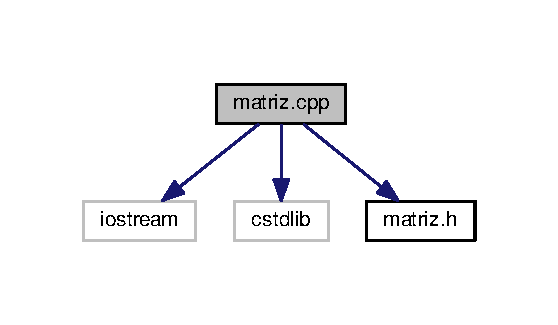
\includegraphics[width=268pt]{matriz_8cpp__incl}
\end{center}
\end{figure}
\subsection*{Functions}
\begin{DoxyCompactItemize}
\item 
\hyperlink{class_matriz}{Matriz} \hyperlink{matriz_8cpp_a909d6a39e8b3be2ae33e3b9209c1b7bf}{operator$\ast$} (float a, const \hyperlink{class_matriz}{Matriz} \&m)
\end{DoxyCompactItemize}


\subsection{Function Documentation}
\index{matriz.\+cpp@{matriz.\+cpp}!operator$\ast$@{operator$\ast$}}
\index{operator$\ast$@{operator$\ast$}!matriz.\+cpp@{matriz.\+cpp}}
\subsubsection[{\texorpdfstring{operator$\ast$(float a, const Matriz \&m)}{operator*(float a, const Matriz &m)}}]{\setlength{\rightskip}{0pt plus 5cm}{\bf Matriz} operator$\ast$ (
\begin{DoxyParamCaption}
\item[{float}]{a, }
\item[{const {\bf Matriz} \&}]{m}
\end{DoxyParamCaption}
)}\hypertarget{matriz_8cpp_a909d6a39e8b3be2ae33e3b9209c1b7bf}{}\label{matriz_8cpp_a909d6a39e8b3be2ae33e3b9209c1b7bf}

\hypertarget{matriz_8h}{}\section{matriz.\+h File Reference}
\label{matriz_8h}\index{matriz.\+h@{matriz.\+h}}
This graph shows which files directly or indirectly include this file\+:\nopagebreak
\begin{figure}[H]
\begin{center}
\leavevmode
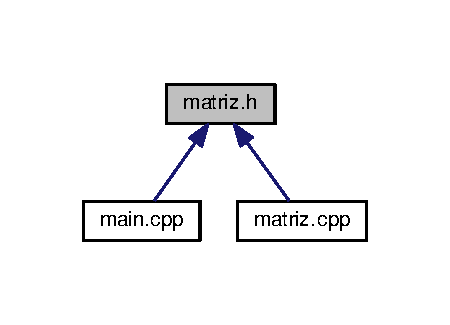
\includegraphics[width=216pt]{matriz_8h__dep__incl}
\end{center}
\end{figure}
\subsection*{Classes}
\begin{DoxyCompactItemize}
\item 
class \hyperlink{class_matriz}{Matriz}
\begin{DoxyCompactList}\small\item\em The \hyperlink{class_matriz}{Matriz} class serve para realizar operacoes matriciais. \end{DoxyCompactList}\end{DoxyCompactItemize}

%--- End generated contents ---

% Index
\backmatter
\newpage
\phantomsection
\clearemptydoublepage
\addcontentsline{toc}{chapter}{Index}
\printindex

\end{document}
